\documentclass[10pt,twocolumn,letterpaper]{article}

\usepackage{cvpr}
\usepackage{times}
\usepackage{epsfig}
\usepackage{graphicx}
\usepackage{amsmath}
\usepackage{amssymb}

% Include other packages here, before hyperref.

% If you comment hyperref and then uncomment it, you should delete
% egpaper.aux before re-running latex.  (Or just hit 'q' on the first latex
% run, let it finish, and you should be clear).
\usepackage[pagebackref=true,breaklinks=true,letterpaper=true,colorlinks,bookmarks=false]{hyperref}

% \cvprfinalcopy % *** Uncomment this line for the final submission

\def\cvprPaperID{****} % *** Enter the CVPR Paper ID here
\def\httilde{\mbox{\tt\raisebox{-.5ex}{\symbol{126}}}}

% Pages are numbered in submission mode, and unnumbered in camera-ready
\ifcvprfinal\pagestyle{empty}\fi
\begin{document}

%%%%%%%%% TITLE
\title{Embracing Uncertainty: Coupling Cascaded Forest Predictors with
Model-based Marginals for Semantic Segmentation}

\author{First Author\\
Institution1\\
Institution1 address\\
{\tt\small firstauthor@i1.org}
% For a paper whose authors are all at the same institution,
% omit the following lines up until the closing ``}''.
% Additional authors and addresses can be added with ``\and'',
% just like the second author.
% To save space, use either the email address or home page, not both
\and
Second Author\\
Institution2\\
First line of institution2 address\\
{\tt\small secondauthor@i2.org}
}

\maketitle
%\thispagestyle{empty}

%%%%%%%%% ABSTRACT
\begin{abstract}
Embracing Uncertainty: Coupling Auto-context predictors with
Model-based Marginals for Spine Localization in Zebrafish

Embracing Uncertainty: Coupling Auto-context predictors with
Model-based Marginals for Semantic Segmentation

   We mix discriminative (discr) and generative models (gen), in a smart way.
\end{abstract}

%%%%%%%%% BODY TEXT
\section{Introduction}
The idea is to do "model-based smoothing" of the output of a Random Forest classifier, in an iterative or cascaded fashion.  This generalizes the idea proposed by GeoF~\cite{GeoForests2013}, which does "image aware" smoothing, using Geodesic distances. 
%
Another way to look at this is that we want to mix discriminative (discr) and generative models (gen), in a smart way.  E.g., The discr model initializes the gen model in the right search space, the gen model then refines this initialization.  This process is iterated while simultaneously increasing the "confidence" in the discr model output. 

Our contributions: 
%
(1) Use Active Appearance Model and HMM for "`image aware"' smoothing in a RF cascade. 
Closest works: 
First, AutoContext~\cite{AutoContext2008}, but they don't do any smoothing. 
Second, GeoF~\cite{GeoForests2013}, but they don't use a generative model for smoothing. 
Third, Glocker~\cite{Glocker2013}, but they do not run a cascade. 
%
(2) Tree weighting based on smoothing. Can be combined with any kind of smoothing. Idea: rate the trees of a forest: who agrees most with the smoothed output? This way, ...
%


Literature.
\begin{enumerate}
\item GeoF~\cite{GeoForests2013}: Geodesic smoothing of RF output.  Uses an Entangled Forest.
\item Deformable Templates Guided Discriminative Models for Robust 3D Brain MRI Segmentation.~\cite{BrainSeg2013}  Liu et al.  2013: Uses generative model to "refine" features in a cascaded discriminative classifier.
\item AutoContext~\cite{AutoContext2008}.  Tu.  2008.
\item Automatic Localization and Identification of Vertebrae in Arbitrary Field-of-View CT Scans.~\cite{Glocker2012} Glocker et al.  2012: Uses Regression Forest.
\item Vertebrae Localization in Pathological Spine CT via Dense Classification from Sparse Annotations.~\cite{Glocker2013} Glocker et al.  2013: Uses Classification this time.
\item Uwe's hint \cite{Denzler2012}: As Time Goes by -- Anytime Semantic Segmentation with Iterative Context Forests
\end{enumerate}

---- SSMs and Random Forests:

Cootes Femur TMI 2013~\cite{CootesFemurTMI2013}

Cootes Regression Forest + SSM ECCV 2012~\cite{CootesECCV2012RRFandSSM}

---- Constellation models and Forests:

Spine: Glocker~\cite{Glocker2013}

Body parts: Auto Context~\cite{AutoContext2008}, "`Pose Machines"' ECCV 2014~\cite{PoseMachinesECCV2014}

Abdominal images: GeoF~\cite{GeoForests2013}, and GeoF at IPMI 2011~\cite{CriminisiAbdominalIPMI2011}: "'Entangled Decision Forests and their Application for Semantic Segmentation of CT Images"'. Seifert SPIE: Marginal space learning classifier plus MRF~\cite{SeifertAnatomicalSPIE2009} 

(Fish: Rotation invariant features, Ronneberger VibeZ)

---- Cascading with Model Fit

DTF, RTF, GeoF

---- Constellation models of self-similar structures

Spine: (Glocker) Klinder (SSM)~\cite{Klinder2009471}: Generalized Hough Transform as detector

Dental: our MICCAI 2012~\cite{TeethMICCAI2012} (Generalized Hough Transform + SSM as detector)

Worm~\cite{WormMiccai2014}

\section{Background}

\subsection{RF}
Filter Bank, Classification Forest, offset and difference features. 

\paragraph{Cascade}

\paragraph{Constellation Model/Inference}
HMM, probabilistic inference.

\subsection{AAM}
Active appearance models (AAMs)~\cite{CootesAAM2001} are linear, generative, parametric models of shape and appearance that are learned (PCA) from training data.  Fitting an AAM is a non-linear optimisation problem, that is done via incremental updates to fitting parameters.  Importantly, AAMs can be easily extended to include priors on the model parameters (see also~\cite{BakerAAM2004}).  

Shape Model:

\[s = s_0 + \sum_{i=1}^n p_i s_i\]

where s is a vector of x,y coordinates of the landmarks that define the shape.  From PCA, $s_0$ is the mean shape, and $s_i$ are n eigenvectors corresponding to the n largest eigenvalues.  Not shown here is that the training data is first noramlised using a Procrustes analysis using a global shape normalising transformation (in our case, a similarity transform) to avoid modeling this variation in the linear model.

Appearance Model:

\[A(x) = A_0(x) + \sum_{i=1}^m \lambda_i A_i(x)\]

Analogous to shape model. $A_0$ and $A_i$ are computed from PCA on a set of \emph{shape normalised} training images, which have been warped onto the base-mesh $s_0$.  Shape normalizing is a key benefit of AAMs (compared to e.g. Eigen-faces), and leads to more compressed PCA representation.

To create a model instance, create an image A(x) (defined by $\lambda$) on the base-mesh, and then warp it to s (defined by p).  Warping is done using a thin-plate spline, parameterized by the set of landmarks, $s_0$ and s.  This defines the unique warp parameterised by p, called W(x;p).

Fitting criteria:

\[Error = A_0(x) + \sum_{i=1}^m \lambda_i A_i(x) - I(N(W(x;p);q)) \]

where N(x;q) is the similarity transform, parameterized by q, and the cost is typically the sum of squared errors over the shape normalized patch.

\[Cost = \sum_{x \epsilon s_0} [Error]^2 \]

Final note, the most efficient fitting routine [] actually "projects out" the appearance variation (from the Error image), and simply solves for the parameters of the transformation: p,q.  If you keep one shape parameter (n=1), this leads to a 5 parameter model.

\paragraph{Priors}

One can add priors on the model parameters, as follows:

\[ \sum_{x \epsilon s_0} [A(x) - I(N(W(x;p);q)]^2 + \sum_{i=1}^K F_i^2(p,q) \]

If $F_i(p,q)$ is quadratic, this can be interpreted in the Bayesian framework as Gaussian Regularization.  There's also a clear way to "ramp" the importance of the priors as:

\[ F_i^2(p,q) = r[(p-p_0)^2+(q-q_0)^2]) \]

where r is the parameter that captures how much we trust the discr model output (this could be learned).

Note, adding priors doesn't slow down the code too much.  You can still use the same fitting algorithm, there's just some extra computation in each loop.


\section{Method: Cascaded RF Interleaved with Probabilistic Generative Constellation Model Inference}
\begin{figure*}[t]
\begin{center}
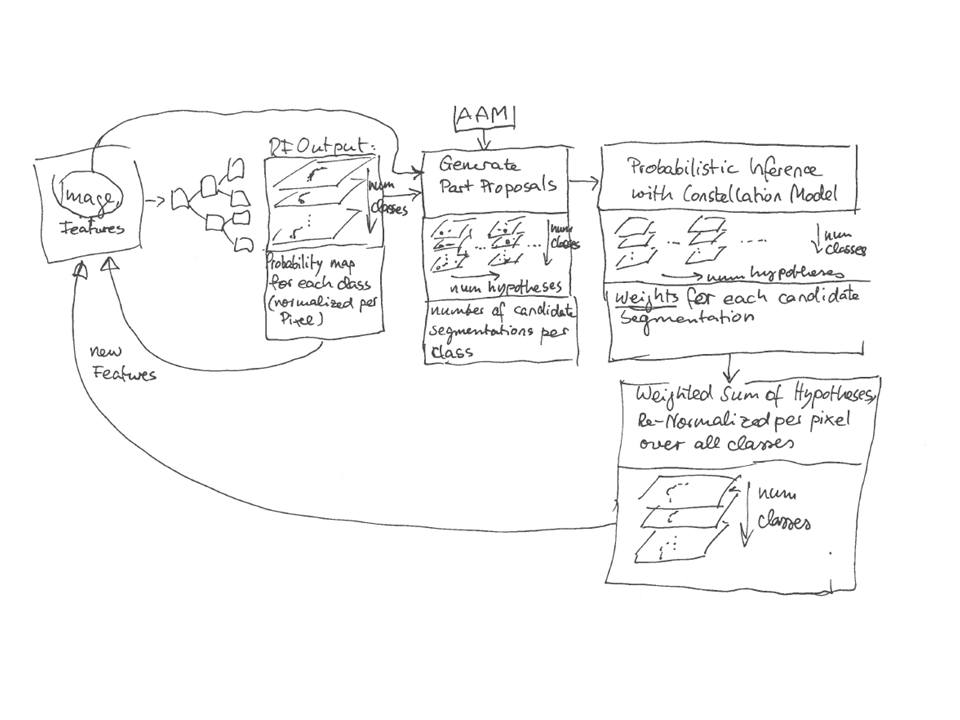
\includegraphics[width=\textwidth]{Pipeline.png} %&[trim=0cm 2cm 0cm 1cm,height=0.2\textheight]
\caption{Pipeline.}
\label{tab:pipeline}
\end{center}
\end{figure*}



By the above method, a number of model instances would be initialized and fit, for each segment.  Each model instance has a cost associated with its fit.  Use these costs as unaries in a Markov Chain Model.  The pair-wise energy comes from statistics on the relative position of neighboring segments in the training data.  This is exactly what Glocker did already; however, we would do probabilistic inference (rather than MAP inference) and keep all the marginals.


The first step is to use the AAM model to fit the grayscale image in a way that is guided by the output of the RF.  There are (at least) two ways to do this: additive and multiplicative.

\subsection{Additive Method}

Simultaneously minimize the error from two AAMs:

\[ \sum_{x \epsilon s_0} [A(x) - I(N(W(x;p);q)]^2 + r\sum_{x \epsilon s_0} [A_2(x) - I_2(N(W(x;p);q)]^2 \]

where $I_2$ is the RF output and $A_2(x)$ is a "soft mask" from averaging all of the ground truth labelings.  Again, r weights the relative importance of the two terms.  I would tend not to include linear appearance variation for the mask, and since the warp parameters are the same as for the original grayscale image, this doesn't introduce any new AAM parameters.

\subsection{Multiplicative Method}

The most efficient optimization method actually proceeds by minizing the following expression, with respect to $\Delta p$ and $\Delta q$:

\[ \sum_{x \epsilon s_0} [A(N(W(x;\Delta p);\Delta q) - I(N(W(x;p);q)]^2 \]

Thus, I think one can introduce the following change, without breaking the optimization algorithm:

\[ \sum_{x \epsilon s_0} [I_3(N(W(x;p);q)]*[A(N(W(x;\Delta p);\Delta q) - I(N(W(x;p);q)]^2 \]

where $I_3 = 1 - r*log(p(c))$, r is again the relative importance parameter, and p(c) is the prob of class c at pixel x.  This is analogous to using a Robust statistic, which is a per-pixel weight; however, it's a bit more complicated, since the mask of weights is dependent on the warp itself, and so needs to updated during fitting.  This suggests it could be a good deal slower to do the fitting (which is true for Robust Stats).

\subsection{Generating a Smoothed RF Output}

Recall, since we initialized many AAMS for fitting, and did probabilistic inference over all of these solutions, we have multiple masks each with its own probability.  I would propose to use a distance function from each instance \emph{s} of the AAM model fits.

\[ \delta (x,s) = \begin{cases} 0, & \mbox{if } x \epsilon \Omega _s \\ d(x, \Omega _s), & \mbox{else} \end{cases} \]

\[ d(x,\Omega _s) = \inf_{y \epsilon \Omega _s} d(x,y) \]

where $\Omega _s$ is the mask associated with instance s.  Then, 

\[ M(s) = 1 - p(s) \] 

\[ Q(x; M(s), \nabla I) = \min_{s} (\delta (x,s) + \nu M(s)) \]

where p(s) is the probability of a given model instance.  The intuition is as follows: If a pixel x is within the mask region corresponding to a highly probable AAM model fit, then it keeps it's probability; however, if it's far from one of these regions, then it's probability would be reduced.  Through the renormalization, this accomplishes the desired smoothing, as in GeoF.

\subsection{Feature Generation vs. Smoothing}

An alternative way to generate an output from the above method, to be fed back into another RF, is to simply "stamp" the masks associated with the above model instances into an image.  This would amount to a weighted average.

\[ p(c) = \sum_{s=1}^S p(c|s)p(s) \]

where there are S model instances initialized, $p(c|s)$ is a mask associated with model instance s, and p(s) is the prob of model instance s from the probilistic inference.

This "stamping" approach is similar to the smoothing above, except it's not mixed with the original RF output.  From the perspective of generating useful features, this seems like an OK idea.  Question: Is smoothing inherently better than this approach?

\subsection{Model Initialisation}

A key aspect of the problem is how to initialize the AAM model for fitting.  This is one of the big challenges of AAMs, since they're local search methods, and a big benefit of using the RF.  However, there doesn't seem to be a "nice" way to initialize the AAM directly from the RF output.  It's easy to think of ways to initialize the XY position directly from the RF output, but how should you initialize orientation, scale, shape, appearance?  There are for sure some \emph{ad hoc} ways, but it doesn't feel very elegant.  This is where it's interesting to contrast regression, which directly gives you the initialization.

\subsection{Parameters}

\begin{itemize}
\item n: \# of shape modes
\item m: \# of appearance modes
\item r: trust in discr output
\item S: \# of model instances that are initialized for fitting
\item g: \# of grad descent steps
\end{itemize}

all parameters could potentially ramp with increasing depth in the cascade to reflect increasing confidence that the model starts in a good search space.  r is potentially most interesting.


\subsection{We get Two Results: RF Output, smoothed Output.}

\subsection{Tree Weights?}

\section{Results}
Approach: Cascade interleaved with "`smoothing"'. 
Evaluation: Different kinds of "`smoothing"', each with different kinds of outputs.

Dataset: 32 images of developing zebrafish. Task: Semantic segmentation of 21 somites (i.e.\ developing vertebrae).

\paragraph{Our Setup: Probabilistic Inference}

\paragraph{Comparison: Auto Context}

\paragraph{Comparison: GeoF}
The simplest way to generate a smoothed RF Output is to re-use the Geodesic smoothing idea from Criminisi.  Let:

\[ Q(x; M, \nabla I) = \min_{x'} (\delta (x,x') + \nu M) \]

and $\nu$ is some free parameter.  Note, x and x' are two points in the image. $M(x') = 1 - p(c|v(x'))$, where v(x') is the feature vector at pixel x'.  Then the smoothed RF output is calculated as:

\[ g(c|v(x)) = \frac{1}{Z} p(c|v(x)) e^{\frac{-Q(x;p(c|v(\Omega)),\nabla J)^2}{\sigma ^2}} \]

This accomplishes smoothing in quite an indirect way, as a competition between different possible class labels for a given pixel, mediated by the normalization Z.  \textbf{It would be interesting to think of more direct ways to implement smoothing.}  However, within this framework, we could just replace the geodesic distance function and the definition of M.


\paragraph{Comparison: MAP Inference}

Experiments:
\begin{enumerate}
\item Auto Context
\item GeoF (two versions)
\item AAM with MAP inference 
\item AAM with probabilistic inference 
\item (AAM with probabilistic inference, tree weighting)
\end{enumerate}

\begin{figure}[t]
\begin{center}
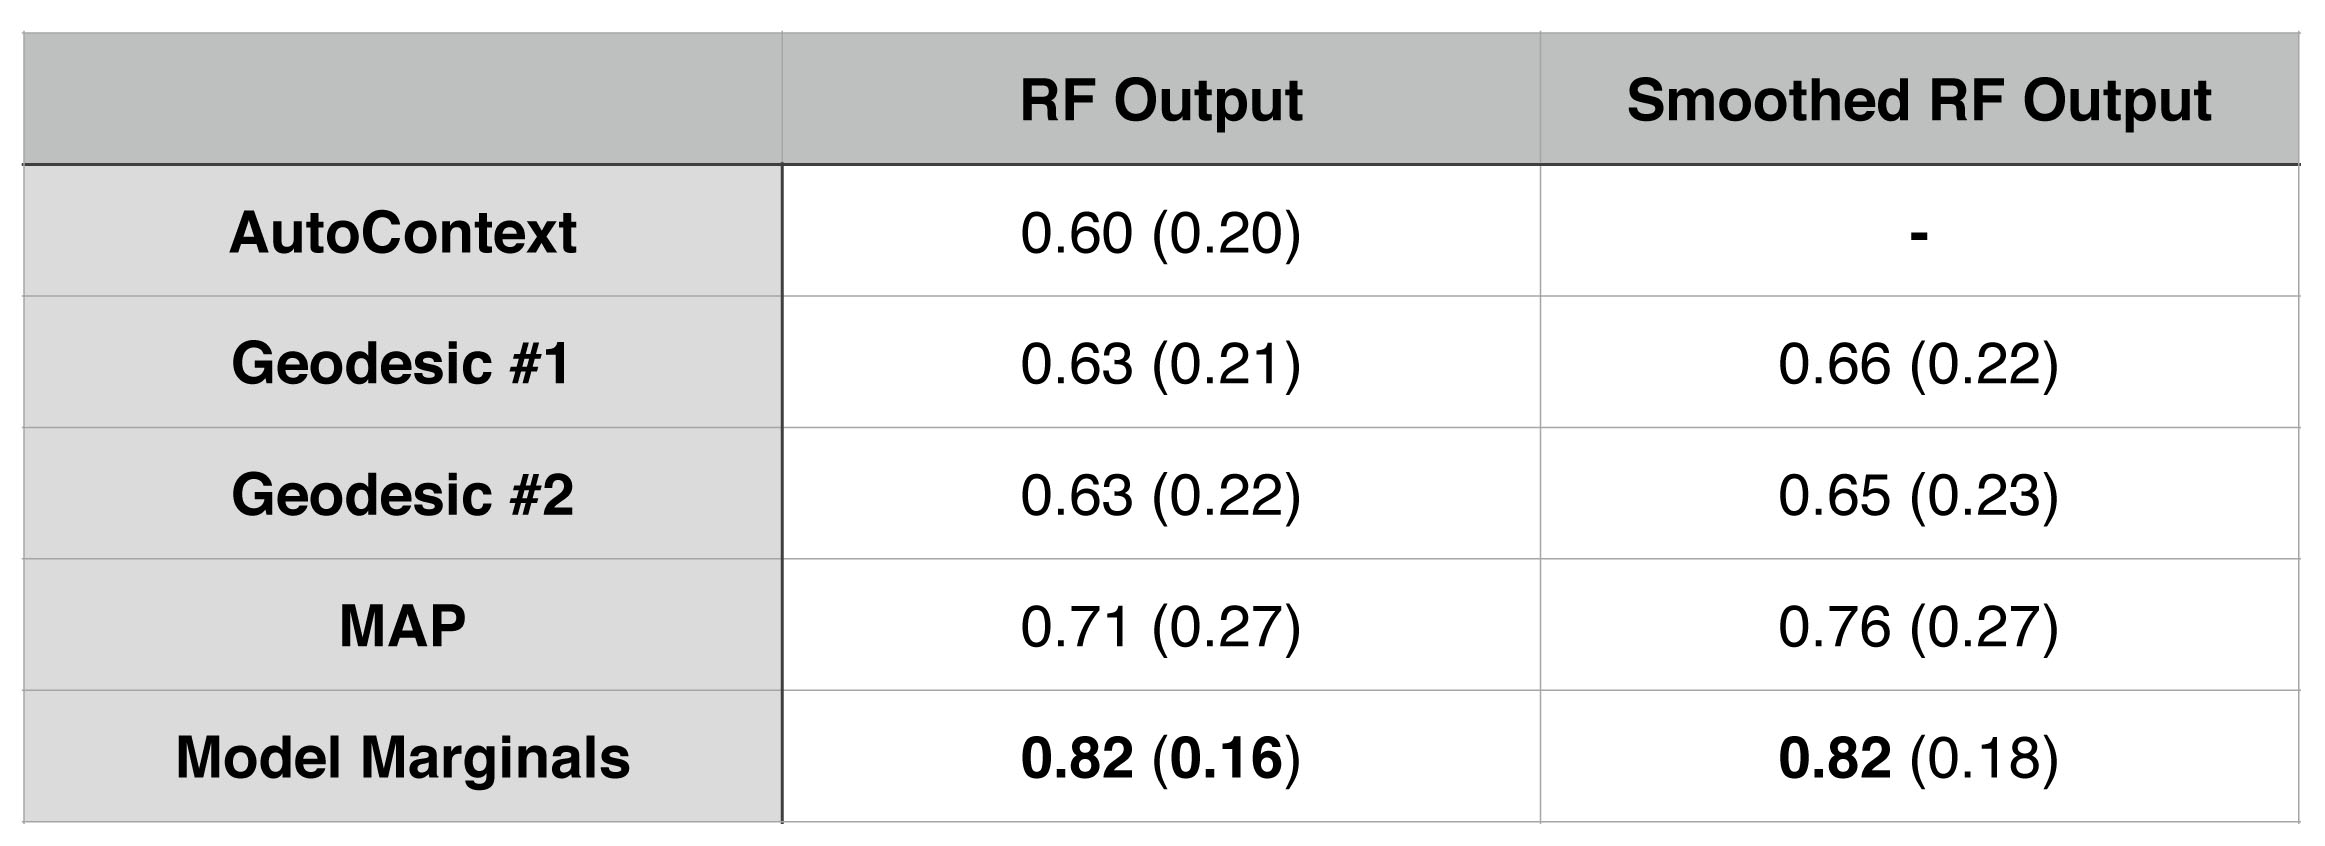
\includegraphics[width=\columnwidth]{TableDiceScores.jpg} %&[trim=0cm 2cm 0cm 1cm,height=0.2\textheight]
\caption{Evaluation on 32 datasets. Dice Scores on all 21 Somites: Mean and standard deviation (in brackets).}
\label{tab:results}
\end{center}
\end{figure}

\begin{figure*}[tb]
\centering
\small
\begin{center}
%	\figpart{a}
		(a) \includegraphics[trim=0cm 2cm 0cm 1cm,height=0.2\textheight]{gfx/boxplot_RF.png} %&
%	\quad
%	\figpart{b}
		(b) \includegraphics[trim=.75cm 2cm 0cm 1cm,height=0.2\textheight]{gfx/boxplot_GeoF.png} \\
%	\,
%	\figpart{c}
		(c) \includegraphics[trim=.75cm 2cm 0cm 1cm,height=0.2\textheight]{gfx/boxplot_model.png} %\\
\end{center}
%\includegraphics[trim=4cm 0cm 5cm 0cm, clip=true, width=0.45\textwidth]{gfx/noInpainting.png} \\
\label{boxplots}
% \vspace{-2mm}
\caption{ %Box plots of Dice scores.}
%\figpart{a}~ 
(a) 2 level cascade, RF output 
%
% \figpart{b}~
(b) geodesic smoothing, 1st level
%
% \figpart{c}~
(c) model fit}
\end{figure*}

\section{Discussion}
Ours is the best :)

\paragraph{Cascading Helps!}
... performance goes up over levels. Boxplots!

... "`traditional"' MAP after one level sucks. 

\paragraph{Smoothing Helps! Model-based Smoothing Helps Best!}
... Auto Context $<$ GeoF $<$ Model Based. Reason: More Specific Prior knowledge...

\paragraph{Uncertainty Helps!}
... Probabilistic inference considerably outperforms MAP inference (6\% better). Reason: With Prob.\ inference, cases can be rescued if not caught after first level (i.e.\ "`at first site"'). Show some rescue cases. 

We also tried MAP after third level. Once all cases are rescued, MAP is fine (performs equally -- state numbers). BUT NOT EARLIER!



{\small
\bibliographystyle{ieee}
\bibliography{somites2014}
}

\end{document}
